\chapter{Experimental overview of rare radiative decays}\label{sec:exp_overview}

There are two main types of analyses which inherit the meaning from their theoretical description presented in \Cref{ch:theory}: \textit{inclusive} analyses and \textit{exclusive} analyses.
Another method, which is a mixture of the two methods, is known as \textit{sum-of-exclusive} method.
Theoeretical motivations for inclusive measurements in terms of \BtoXsgamma have already been discussed in \Cref{sec:btosgamma_totalrate_theory,sec:btosgamma_spectrum_theory}.
Similar motivations hold true for other electroweak decay channels such as, $B\to X_s\ell\bar{\ell}$ ($\ell\in\{\mu^-,e^-,\nu\}$).
However, compared to the latter, $B\rightarrow X_s\gamma$ contains one less interaction vertex and therefore is enhanced by $\sim\alpha_{\mathrm{em}}$, which makes it experimentally acessible with smaller datasets.
In this chapter, I will introduce the main methods of performing an inclusive measurement, while focusing solely on \BtoXsgamma, although, generally, these methods are applicable for other decay channels as well.

\section{Past measurements of \safeBtoXsgamma decays}

Inclusive measurements target to measure a wide selection of decay products; in the case of $X_{sd}$, the sum of all states that originate in $b\to s$ or $b\to d$ transitions.
In principle, such states include resonant and non-resonant states.
A notable resonant state is $B\rightarrow \Kstar(892)\gamma$.
Experimentally it is highly-accessible due to its narrow and isolated peak near the $b\to s\g$ two-body decay kinematic limit.
A similar state for $b\rightarrow d\g$ is the $B\rightarrow \rho(770)\gamma$.
Non-resonant states include combinations of one or more pions and, in case of $b\rightarrow s$, kaon.
While the goal of an inclusive measurement is to measure the energy of photons from all these decays simultaneously, an exclusive measurement attempts to select one or several particular states from the spectrum.

The world-average values of inclusive radiative $B$ decay measurements are~\cite{Amhis:2022mac,Workman:2022ynf}:
\begin{align}\label{eq:btosgamma_experimental}
    \begin{split}
    \mathcal{B}(\BtoXsgamma)=(3.49\pm 0.19)\times10^{-4}\\
    \mathcal{B}(\BtoXdgamma)=(0.09\pm 0.03)\times10^{-4}.
    \end{split}
\end{align}
The values of \Cref{eq:btosgamma_experimental} can be compared to the theoretical prediction in \Cref{eq:btosgamma_theoretical,eq:btodgamma_theoretical}.
\BtoXsgamma results show an excellent agreement between the theory and experiment.
For \BtoXdgamma, values agree within $2\sigma$, however, the experimental uncertainty is dominated statistically 
and performed using the \textit{sum-of-exclusive} approach, which may explain the lower value due to unaccounted $b\rightarrow d\gamma$ modes in the simulation.

\Cref{tab:btosgamma_bfs} provides the experimental status of observed most prominent \BtoXsdgamma decay channels as of December 2022.
Due to final-state similarity and overlap between various resonant and non-resonant decay modes, only the most prominent resonant decays have been measured.
However, even in the case of a relatively islolated decay channel such as \BtoKstargamma, the overall precision of inclusive measurements is higher (compare to \Cref{eq:btosgamma_experimental}).

{\renewcommand{\arraystretch}{1.2}
\begin{table}[!htbp]
    \centering
    \caption{\label{tab:btosgamma_bfs} 
    Branching fractions of \BtoXsgamma modes for charged and neutral modes.
    The table only includes decay modes that have been observed and (for $\BtoXsgamma$ only) have a branching fraction $\gtrsim10^{-5}$.
    The \Bp decays are ordered in terms of the experimental precision $\mathcal{B}/\Delta\mathcal{B}$, whereas \Bz are ordered in relation to \Bp, where applicable.
    The values correspond to the averages of experimental measurements given in Refs. \cite{Amhis:2022mac,Workman:2022ynf}.
    }
    \begin{minipage}[c]{0.5\textwidth}
    \centering
    \BptoXsgamma exclusive modes
    \resizebox{1\textwidth}{!}{
    \begin{tabular}{|lc|}
        \hline
        Decay mode & Branching fraction ($\times 10^{-4}$) \\
        \hline
        \multicolumn{2}{|c|}{\textbf{Two decay products}}\\
        $\Bp \to \Kstar(892)^+ \gamma$  & $0.392 \pm 0.022$ \\
        $\Bp \to K_1(1270)^+  \gamma$   & $0.438 \pm ^{0.071}_{0.063}$ \\
        $\Bp \to K_2^*(1430)^+  \gamma$ & $0.138 \pm 0.040$ \\            
        $\Bp \to K^*(1410)^+  \gamma$   & $0.271 \pm ^{0.080}_{0.061}$ \\
        $\Bp \to K^*(1680)^+  \gamma$   & $0.670 \pm ^{0.170}_{0.140}$ \\
        $\Bp \to K_1(1400)^+  \gamma$   & $0.097 \pm ^{0.054}_{0.038}$ \\
        \hline
        \multicolumn{2}{|c|}{\textbf{Three or more decay products}}\\
        $\Bp \to \Kstar(892)^0 \pi^+ \gamma$ & $0.233 \pm 0.012$ \\
        $\Bp \to K^+ \pi^+\pi^- \gamma$ & $0.258 \pm 0.015$ \\
        $\Bp \to K^0 \pi^+\pi^0 \gamma$ & $0.456 \pm 0.052$ \\
        $\Bp \to K^+ \pi^+\pi^- \gamma$ (non-resonant) & $0.099 \pm ^{0.017}_{0.020}$ \\
        \hline
    \end{tabular}
    }
\end{minipage}
\begin{minipage}[c]{0.395\textwidth}
    \centering
    \BztoXsgamma exclusive modes
    \resizebox{1\textwidth}{!}{
    \begin{tabular}{|lc|}
        \hline
        Decay mode & Branching fraction ($\times 10^{-4}$) \\
        \hline
        \multicolumn{2}{|c|}{\textbf{Two decay products}}\\
        $\Bz \to \Kstar(892)^0 \gamma$ & $0.418 \pm 0.025$ \\
        - & -\\
        $\Bz \to K_2^*(1430)^0 \gamma$ & $0.124 \pm 0.024$ \\ 
        - & -\\
        - & -\\
        - & -\\
        \hline
        \multicolumn{2}{|c|}{\textbf{Three or more decay products}}\\
        - & -\\
        $\Bz \to K^+ \pi^-\pi^0 \gamma$ & $0.407 \pm 0.038$\\
        $\Bz \to K^0 \pi^+\pi^- \gamma$ & $0.199 \pm 0.018$\\
        - & -\\
        \hline
    \end{tabular}
    }
\end{minipage}

\vspace{10pt}

\begin{minipage}[c]{0.395\textwidth}
    \centering
    $B\to X_d\gamma$ exclusive modes
    \resizebox{1\textwidth}{!}{
    \begin{tabular}{|lc|}
        \hline
        Decay mode & Branching fraction ($\times 10^{-4}$) \\
        \hline
        $\Bp \to \rho^+(770)\gamma$ & $0.0098 \pm ^{0.0025}_{0.0024}$\\
        $\Bz \to \rho^0(770)\gamma$ & $0.0086 \pm 0.0015$\\
        $\Bz \to \omega(782)\gamma$ & $0.0044 \pm ^{0.0018}_{0.0016}$\\
        \hline
    \end{tabular}
    }
\end{minipage}

\end{table}
}

Currently, inclusive measurements are only attainable at $B$ factories.
The relatively low-background environment offered by an $\epem$ collision allows to treat the $X_{sd}$ system as a `missing-energy' system with no explicit requirements.
Although the process of event reconstruction and detection by itself may introduce a bias to the inclusive system, this is expected to be a much smaller effect than other experimental factors, such as resolution and poissonian fluctations.
Conversely, at hadron colliders, large probability for multiple proton pairs interacting in a collision event creates a large QCD background, usually referred to as \textit{pileup}.
This makes it complicated to select an unbiased and model independent inclusive sample and,
at the time of writing this, no inclusive $B$ measurement has been performed outside of a $B$-factory experiment.

Even in the case of exclusive radiative measurements, such as $B\rightarrow \Kstar\gamma$, $B$-factory have historically outperformed hadron collider experiments (such as LHCb) due to a higher-degree of control of combinatorial background.
Final states that include neutral particles and photons are problematic to measure accurately in high pileup conditions.
Therefore, with several exceptions (e.g. \cite{Bellee:2019qbt}), the field of rare radiative $B$ decay measurements is dominantly probed by $B$-factory experiments.



\section{Techniques for inclusive \safeBtoXsgamma measurements}\label{sec:btosgamma_techniques}
Historically, three different techniques were applied for inclusive \BtoXsgamma analyses at $B$ factories: 
sum-of-exclusive measurements,
untagged-inclusive measurements,
tagged-inclusive measurements.

The summary of the most-precise measurements that are used in experimental average in \Cref{eq:btosgamma_experimental} is given in \Cref{tab:btosgamma_inclusive_summary}.
These experiment techniques are explained in more details in this Section.
The primary focus will be given to the hadronic-tagged technique, which is applied for the measurement described in this thesis.

{\renewcommand{\arraystretch}{1.2}
 \begin{table}[!htbp]
     \centering
     \caption{\label{tab:btosgamma_inclusive_summary}
     The table shows the experiments and their most-precise results from various techniques of measuring \BtoXsgamma.
     These results are included in the total \BtoXsgamma average (\Cref{eq:btosgamma_experimental}) \cite{Amhis:2022mac,Workman:2022ynf}.
     The thresholdd of the photon energy in the decaying $B$-meson rest-frame (\EB), quoted in corresponding papers, are also provided.
     The measurements had differing thresholds, however, their branching fractions are given as extrapolated to 1.6~\gev, using extrapolation factors calculated in Ref. \cite{Buchmuller:2005zv}.
     Belle$^{\dagger}$ measurement was not published or used in the averages, but is included here as the lepton-tagged measurement with largest data sample.
     }
     \resizebox{1.\textwidth}{!}{
\begin{tabular}{lllllc}

Year & Experiment                 & Technique & Data used  & Energy threshold &  $\mathcal{B}(B\rightarrow X_s\gamma) \times 10^{-4}$  [$\EB>1.6~\gev$]\\ 
\hline
2001 & CLEO  \cite{CLEO:2001gsa}  & Untagged         & 9.1~\invfb &  $\EB>2.0~\gev$ & $3.29\pm0.44\pm0.29$\\ 
2007 & BaBar \cite{BaBar:2007yhb} & Hadronic-tagged  & 210~\invfb &  $\EB>1.9~\gev$ & $3.90\pm0.91\pm0.64$\\ 
2009 & Belle \cite{Belle:2009nth} & Untagged/Lepton-tagged      & 605~\invfb &  $\EB>1.7~\gev$ & $3.47\pm0.15\pm0.40$\\ 
2012 & BaBar \cite{BaBar:2012fqh} & Lepton-tagged         & 347~\invfb &  $\EB>1.7~\gev$ & $3.32\pm0.16\pm0.31$\\ 
2012 & BaBar \cite{BaBar:2012eja} & Sum-of-exclusive & 429~\invfb &  $\EB>1.7~\gev$ & $3.52\pm0.20\pm0.51$\\ 
2014 & Belle \cite{Belle:2014nmp} & Sum-of-exclusive & 711~\invfb &  $\EB>1.7~\gev$ & $3.75\pm0.18\pm0.35$\\
2016 & Belle$^{\dagger}$ \cite{Belle:2016ufb} & Lepton-tagged & 711~\invfb & $\EB>1.6~\gev$ & $3.12\pm0.10\pm0.21$\\
%\hline
%2022 & {\bf Belle II}& Hadronic               & 189 fb$^{-1}$ & $3.54 \pm0.78 (\mathrm{stat.})\pm0.83(\mathrm{syst.})$ &              $E^B_{\gamma}>1.8~\gev$                 \\
\end{tabular}
}
 \end{table}
 }

\subsection{Sum-of-exclusive technique}\label{sec:sum_of_exclusive}

Sum-of-exclusive measurement technique embodies the idea of reconstructing `all $X_s$ states' separately and summing them up into an inclusive spectrum.
In practice, this is, of course, impossible and previous BaBar and Belle analyses (\cite{BaBar:2012eja,Belle:2014nmp}) reconstruct an sum 38 exclusive channels, that amount to roughly 70\% of the total \BtoXsgamma decay width.
The exclusive final states include various combinations of one or multiple $K^{\pm}$, $K_S^0$, $\pi^{\pm}$, $\piz$, $\eta$.
Modes with up to two three kaons, four pions and one $\eta$-meson are considered.


Evidently, a significant challenge following from this treatment is the proper treatment of \BtoXsgamma events that have been incorrectly reconstructed in one of the 38 final states.
Photons originating in non-\BtoXsgamma decay chains, particularly decays of type $B\to D^{(*)}\rho^+$ and non-$B$ events, also contribute significantly as background.
Much more than in the case of `inclusive' measurements, this technique depends strongly on the $X_s$ fragmentation modelling, which has to be be carefully tuned and calibrated to best represent experimental data.
Finally, a measurement performed this way is only `pseudo-inclusive', meaning that additional uncertainties for unaccounted decay phase-space are incurred.


The main advantages are due to precise knowledge of the $X_s$ system, which gives additional information about the $B$-meson, and a higher-degree of control of background.
The knowledge of the charge and flavour of the decaying $B$-meson enables the measurement of the CP and isospin asymmetries \cite{BaBar:2014czi}.
It is the only inclusive measurement technique that has been able to distinguish $X_s$ and $X_d$ states experimentally \cite{BaBar:2010vgu}.
Direct reconstruction of the mass of the $X_s$ system, $M_{X_s}$, and decaying $B$ meson mass is obtained allows to express the photon energy directly in the signal $B$-meson rest frame:
\begin{equation}\label{eq:mx_egamma_relation}
    \EB = \frac{M_B^2 - M_{X_s}}{2M_B},
\end{equation}
which is otherwise only directly obtainable by hadronic-tagged inclusive measurements (see \Cref{sec:had_tagged_overview}).
Furthermore, the full reconstruction of the candidate $B$-meson allows to utilise the well-defined initial state of the \epem collision in additional background suppression.
Two observables can be defined:
\begin{equation}\label{eq:deltae_inclusive}
    \Delta E \equiv E^*_B - \sqrt{s}/2,
\end{equation}
known as energy difference, expressed in terms of the energy of the $B$-meson in the collision center-of-mass frame, $E^*_B$, and
\begin{equation}\label{eq:mbc_exclusive}
    M_{bc} \equiv \sqrt{(\sqrt{s}/2)^2 - (p^*_B)^2},
\end{equation}
known as the beam-constrained mass, expressed in terms of the momentum of the $B$-meson in the collision center-of-mass frame, $p^*_B$.
From \Cref{eq:deltae_inclusive,eq:mbc_exclusive} it is clear that $B$ candidates which are reconstructed correctly tend to have a resonant behaviour in \Mbc and \DeltaE, with their distributions peaking at nominal $B$ mass $\approx5.28~\gevcc$ and $0$, respectively.
The backgrounds tend to have broader or even non-peaking shapes. 
The \Mbc distribution, as seen by the Belle sum-of-exclusive measurement \cite{Belle:2014nmp}, in \Cref{fig:mbc_sum_of_exclusive}.
In the past, these analysis techniques achieved an average signal efficiency of 3.5\%~ (larger for greater values of \EB), after correcting for missing $X_s$ modes \cite{Belle:2014nmp}.

\begin{figure}[htbp!]
    \centering
    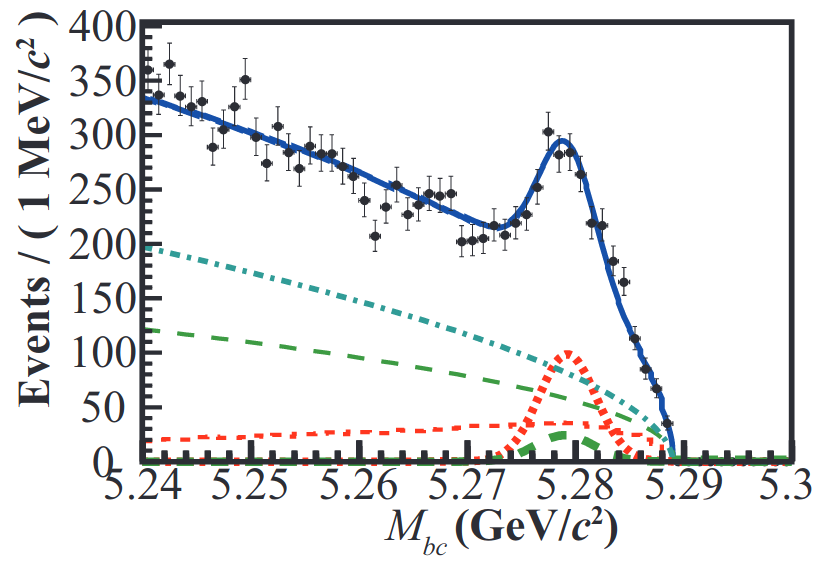
\includegraphics[width=0.4\textwidth]{figures/experiment_overview/Mbc_sum_exclusive_Belle.png}
    \caption{\label{fig:mbc_sum_of_exclusive} 
    The distribution of \Mbc, as seen in the $1.9>M_{X_s}>1.8~\gevcc$ interval by Ref.\cite{Belle:2014nmp} in the sum-of-exclusive state analysis.
    The datapoints are fitted with in an unbinned maximum likelihood fit with a combination of fit functions for 
    signal events (red, thick and short dashed), 
    cross-feed (red, thin and short dashed), 
    peaking $\BB$ (green, thick and long dashed), 
    non-peaking $\BB$ (green, thin and long ashed)
    and $\qqbar$ background events (blue, dash-dotted).
    }
\end{figure}

\subsection{Untagged technique}\label{sec:untagged}
The untagged inclusive measurements, conceptually, are the simplest as they only required a high-energy photon in the final state, without any explicit assumptions about the $X_s$ or partner-$B$ meson decay.
Such a simple requirement guarantees that photons from all $\BtoXsgamma$ decays are included in the selected data sample.
Because any partner-$B$ meson state is accepted, they are sometimes also called \textit{inclusive-tagged} or \textit{fully-inclusive}.
I opt to use \textit{untagged} to stress the difference between the signal-$B$ decay and the partner-$B$.

Although the concept of this technique is simple, the measurement is experimentally highly-challenging.
In particle collision and subsequent processes, high-energy photons can originate in an uncountable number of ways, such as initial \epem state radiation, \epem\ra\qqbar decays, $B$ decays etc.
In the previously introduced \Cref{sec:sum_of_exclusive} technique, this problem is solved by using the information of decays of $X_s$ and utilising observables such as \Mbc and \DeltaE to reduce incorrect photon-candidates. 
Conversely, in the inclusive case the $X_s$ is treated in a missing-mass way, and therefore the background suppression procedure must be performed such that no selection bias is introduced to the $X_s$ system.
An example spectrum based on Belle~II simulation is shown in \Cref{fig:untagged_btosgamma_background}, which highlights signal-to-background difference.

The predominant background originates from events where no $B$-mesons are created: particularly $\epem\to\qqbar$ events ($q={u,d,s,c}$), where a \piz is created through hadronisation and decay of hadrons.
The \piz then decay asymmetrically into two photons, which mimics the isolated high-energy photon of \BtoXsgamma decays.
In particular, $q={u,c}$ processes contribute strongly, due to the fact that they tend to produce energetic \piz or charm-mesons (which subsequently decay to \piz).
Semileptonic and hadronic $B$ decays, that produce \piz, $\eta$ and $\rho$ mesons (whose decays chains involve high-energy photons as described), are among also among the main sources of background contribution.

The usual way to perform this analysis involves the usage of boosted-decision trees or alternative multivariate methods (see \Cref{sec:classification}) to suppress highly-prominent backgrounds.
For example, the technique applied in \cite{CLEO:2001gsa,Belle:2009nth} combines the high-energy photons with all other photons in the event and vetoes those that are compatible with \piz or similar decays.
The contribubutions from \epem\ra\qqbar are suppressed by parametrising the different decay topologies that are are observed for \BB and \qqbar events (see \Cref{sec:continuum_suppression}).
Data samples, collected below the \FourS resonance, which contain only $\epem\ra\qqbar$ events are used to subtract the non-\BB contributions left after the background treatment, 
whereas the \BB contribution is usually removed using simulation.
An example result of extracted \BtoXsgamma spectrum from Belle~II data using $63.1~\invfb$, which is a work that I was involved during my PhD studies, is shown in \Cref{fig:untagged_btosgamma_measured} \cite{Collaboration:2302}.

The strength of the untagged technique is the `truly' inclusive approach, which ensures that all $X_s$ states are selected, as well as a large selection efficiency.
Previous analyses (e.g. \cite{Belle:2009nth}) report an average selection efficiency in their final sample of $\sim 10\%$ (increasing with photon energy), which is several times higher even than the sum-of-exclusive approach.
On the other hand, the missing kinematic information of the $X_s$ system yields a complicated and inefficient background suppression process, which means that such measurements have a small signal-to-background ratio.
Moreover, the kinematic information of the $B$-decay cannot be accessed, which only allows a mesurement of the photon energy in the \epem collision frame.
To reach the theoretically more desirable $B$-meson decay frame, additional modelling uncertainties have to be attached.

\begin{figure}[htbp!]
    \centering
    \subcaptionbox{\label{fig:untagged_btosgamma_background}}{
        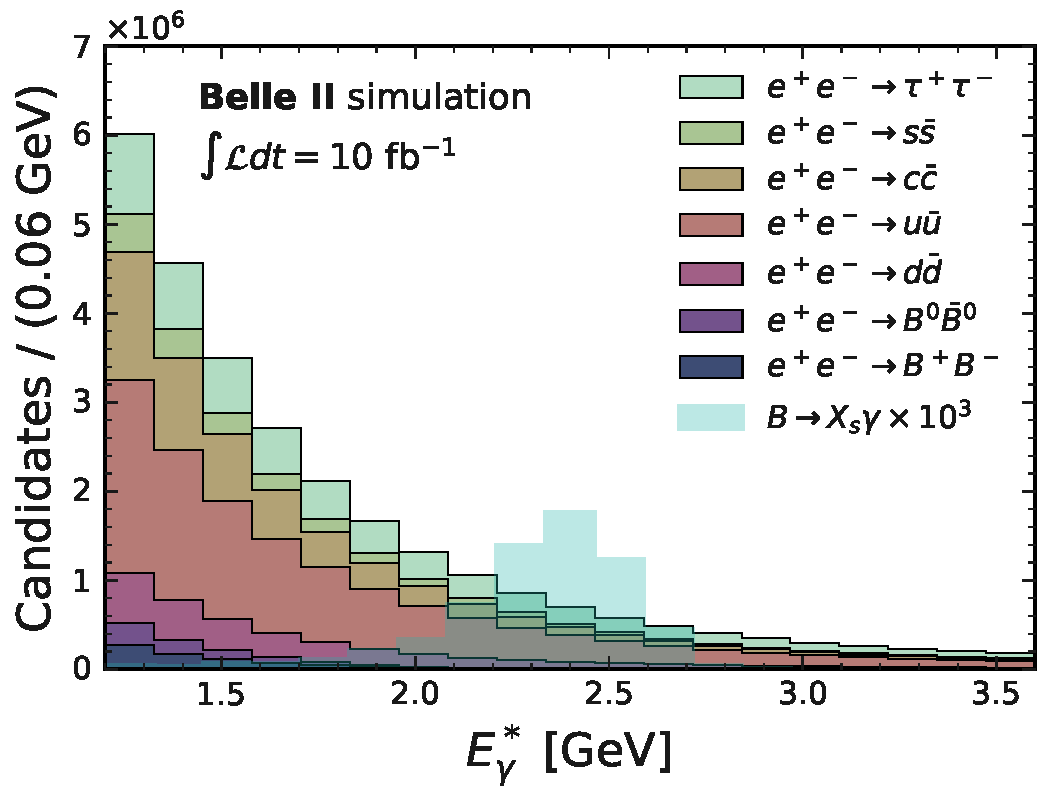
\includegraphics[width=0.45\textwidth]{figures/experiment_overview/untagged_background.pdf}
        }
    \subcaptionbox{\label{fig:untagged_btosgamma_measured}}{
    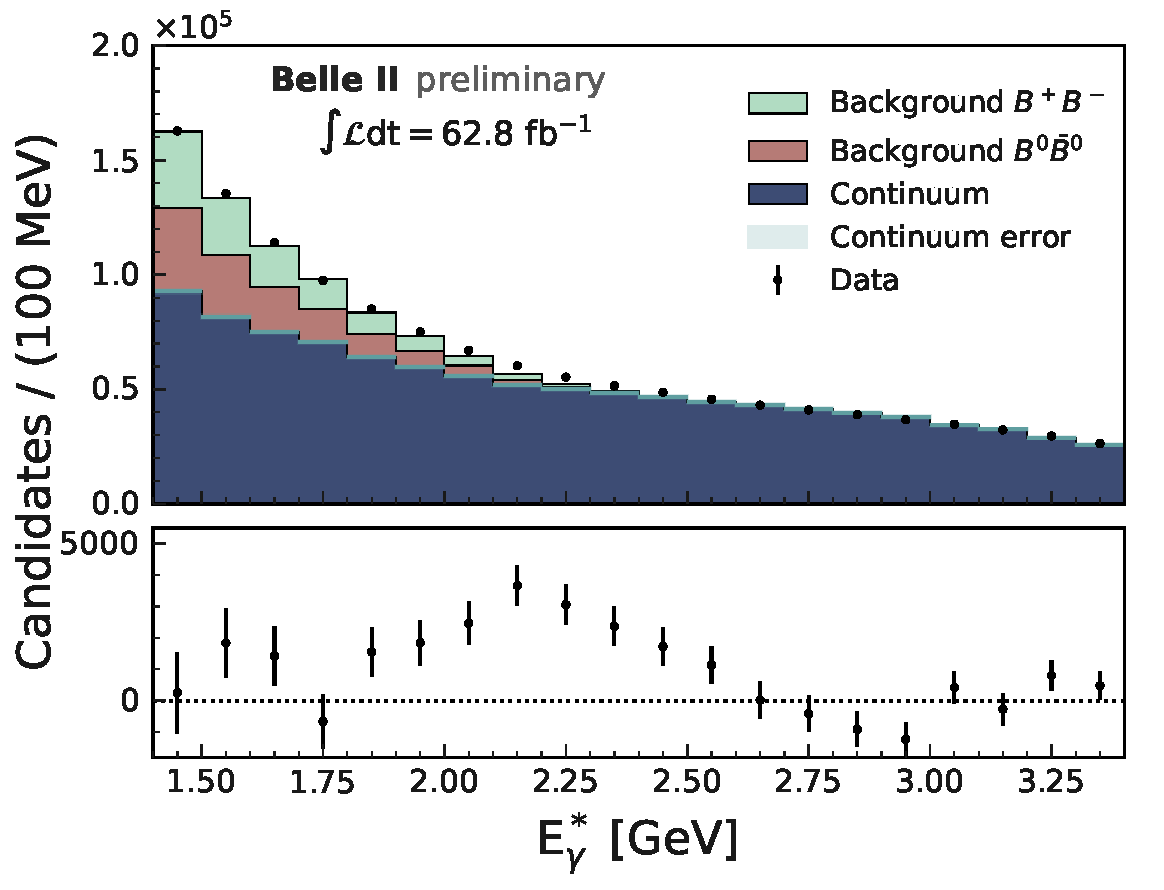
\includegraphics[width=0.45\textwidth]{figures/experiment_overview/untagged_btosgamma.pdf}
    }
    \caption{\label{fig:untagged_btosgamma}Photon energy spectra in \BtoXsgamma decays before (\Cref{fig:untagged_btosgamma_background}) and after (\Cref{fig:untagged_btosgamma_measured}) background suppression.
    Before the background suppression is performed, the signal needs to be amplified by a factor of 1000 to be visible.
    After background suppression, subtracting the remaining continuum (\epem\ra\qqbar decays) and \BB background yields the \BtoXsgamma spectrum (bottom panel).
    Both plots show Belle II simulation, whereas the plot on the right also includes official Belle II data from Ref.\cite{Collaboration:2302}.
    The \Cref{fig:untagged_btosgamma_background} includes a small amount of simulation and was produced for illustrative purposes only. 
    }
\end{figure}

\subsection{Tagged techniques}\label{sec:had_tagged_overview}

To overcome multiple of the issues that come with the untagged measurements presented in \Cref{sec:untagged}, while still selecting an inclusive $X_s$ sample (opposed to \Cref{sec:sum_of_exclusive}), 
additional information pertaining to the second $B$ meson from the \FourS decay can be utilised.
The naming and the idea stems from the widespread \textit{tag-and-probe} methods.
In this approach, the partnerring $B$ meson is fully reconstructed or some of its decay products are identified.
This $B$ meson will henceforth be referred to as \textit{tag}-$B$ meson.
The application of kinematic constraints on the event arising from the tag-$B$ is called \textit{tagging}.
The schematic idea of tagging is shown in \Cref{fig:tagging_schematic}.

There are three main tagging-techniques that have been used in the past at $B$ factories:
\begin{itemize}
    \item \textit{lepton-tagging}, where a lepton, originating from tag-$B$ decays is reconstructed;
    \item \textit{semileptonic-tagging}, where the tag-$B$ is reconstructed as semileptonic $B$ decay, of the form $B\to D^{(*)}\ell\bar{\nu}$;
    \item \textit{hadronic-tagging}, where the tag-$B$ is reconstructed as a decay that involves hadrons in the final state $B\to\mathrm{hadrons}$, such as $B\to K\pi$.
\end{itemize}
The main advantages of these techniques are summarised in \Cref{fig:tagging_advantages}.

\begin{figure}[htbp!]
    \centering
    \subcaptionbox{\label{fig:tagging_schematic}}{
        \resizebox{0.2\textwidth}{!}{
            \pgfdeclarelayer{bg}    % declare background layer
\pgfsetlayers{bg,main}  % set the order of the layers (main is the standard layer)
\begin{tikzpicture}[rotate=90]

    % NODES
    
    % Initial state
    \node [circle, minimum size=1.2cm, draw=white, ultra thick]    (collision) {} ;
    % \node [] (collision) {} ;
    \node [] (collisiontext) [below=0.03cm of collision.west] {\FourS};
    \node [] (eminus)     [left=2cm of collision.center] {};
    \node [] (eplus)     [right=1.5cm of collision.center] {};
    \node [] (eplusabove) [above=0.1cm of eplus] {};
    \node [] (eminusabove) [above=0.1cm of eminus] {};
    \node [] (eminustext)     [right=0.3cm of eminusabove, text=blue] {\en};
    \node [] (eplustext)     [left=0.3cm of eplusabove, text=red] {\ep};
    
    % BB bar
    \node [] (bbarup) [above=0.7cm of collision.north east] {};
    \node [] (bbardown) [below=0.5cm of collision.south east] {};
    \node [] (bbarup_text) [right=0.05cm of bbarup.center] {$\B_{\mathrm{sig}}$};
    \node [] (bbardown_text) [right=0.05cm of bbardown.center] {$\B_{\mathrm{tag}}$};
    
    % Xs gamma
    %%gamma
    \node [] (gamma_int) [left=0.5cm of bbarup.center] {};
    \node [] (gamma) [above=1cm of gamma_int.center] {};
    \node [] (gammatext) [left=0.05cm of gamma.center] {$\gamma$};
    %%xs
    \node [] (Xs_int) [right=0.5cm of bbarup.center] {};
    \node [] (Xs) [above=0.5cm of Xs_int.center] {};
    \node [] (Xstext) [left=0.05cm of Xs.center] {$X_{s}$};
    %%xs daughters
    \node [] (Xsd1_int) [left=0.05cm of Xs.center] {};
    \node [] (Xsd1) [above=0.5cm of Xsd1_int.center] {};
    \node [] (Xsd2_int) [right=0.2cm of Xs.center] {};
    \node [] (Xsd2) [above=0.4cm of Xsd2_int.center] {};
    \node [] (Xsd3_int) [right=0.35cm of Xs.center] {};
    \node [] (Xsd3) [above=0.2cm of Xsd3_int.center] {};
    
    % Tag side
    
    % first generation
    \node [] (D0_int) [left=0.35cm of bbardown.center] {};
    \node [] (D0) [below=0.65cm of D0_int.center] {};
    \node [] (pi0_int) [right=0.3cm of bbardown.center] {};
    \node [] (pi0) [below=0.6cm of pi0_int.center] {};
    
    %second generation
    \node [] (Kp_int) [left=0.25cm of D0.center] {};
    \node [] (Kp) [below=0.65cm of Kp_int.center] {};
    \node [] (pim_int) [right=0.1cm of D0.center] {};
    \node [] (pim) [below=0.6cm of pim_int.center] {};

    \node [] (g1_int) [left=0.2cm of pi0.center] {};
    \node [] (g1) [below=0.65cm of g1_int.center] {};
    \node [] (g2_int) [right=0.15cm of pi0.center] {};
    \node [] (g2) [below=0.6cm of g2_int.center] {};
    
    %\node [] (hadron text) [below=0.05cm of bbardown.center] {\scriptsize hadrons};
    
    % Colored overal blocks
    
    \node [] (sigside) [above=0.8cm of bbarup] {};
    \node [] (tagside) [below=0.8cm of bbardown] {};
    \node [] (tagside_right) [right=0.2cm of tagside] {};
    
    \node [] (sigsidetext) [above=0.1cm of sigside] {\scriptsize Signal side};
    \node [] (tagsidetext) [below=0.3cm of tagside_right, text width = 2cm] {\centering\scriptsize Tag side};
    
    \begin{pgfonlayer}{bg}    % select the background layer
    \node [rectangle, fill=green!20, text width=2cm, text centered, rounded corners, minimum height=1.7cm] (Signal_Side) at (sigside) {};
    \node [rectangle, fill=blue!20, text width=2cm, text centered, rounded corners, minimum height=1.7cm] (Signal_Side) at (tagside) {};
    \end{pgfonlayer}

    

    
    % LINES
    
    % Initial state
    \draw [-Triangle, blue, thick] (eminus) -- (collision.center);
    \draw [-Triangle, red, thick] (eplus) -- (collision.center);
    
    % BB bar
    \draw[-Triangle, thick] (collision.center) -- (bbarup.center);
    \draw[-Triangle, thick] (collision.center) -- (bbardown.center);
    
    % Xs gamma
    \draw[-Triangle, thick, purple, dashed] (bbarup.center) -- (gamma.center);
    \draw[-Triangle, thick] (bbarup.center) -- (Xs.center);
    \draw[-Triangle, thick] (Xs.center) -- (Xsd1.center);
    \draw[-Triangle, thick] (Xs.center) -- (Xsd3.center);
    \draw[-Triangle, thick] (Xs.center) -- (Xsd2.center);
    
    % Tag side
    \draw[-Triangle, thick] (bbardown.center) -- (D0.center);
    \draw[-Triangle, thick] (bbardown.center) -- (pi0.center);

    \draw[-Triangle, thick] (D0.center) -- (Kp.center);
    \draw[-Triangle, thick] (D0.center) -- (pim.center);
    \draw[-Triangle, thick, dashed] (pi0.center) -- (g1.center);
    \draw[-Triangle, thick, dashed] (pi0.center) -- (g2.center);
    

    
\end{tikzpicture}
            }
    }
    \subcaptionbox{\label{fig:tagging_advantages}}{
    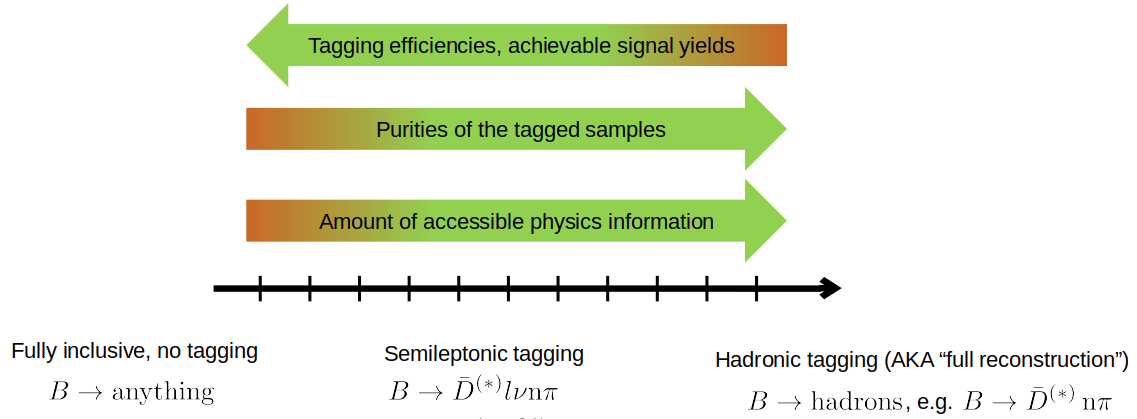
\includegraphics[width=0.6\textwidth]{figures/experiment_overview/tagging_advantages.png}
    }
    \caption{\label{fig:tagging_drawins} Schematic representation of tagging is shown in \Cref{fig:tagging_schematic}.
    The idea of tagging is the usage of the tag-side $B$ decay products to apply kinematic constrains on the signal-side $B$ decay (\BtoXsgamma in the example).
    \Cref{fig:tagging_advantages} highlight the advantages and disadvantages related to the usage of different $B$ decay products for tagging at $B$-factories.
    A detailed discussion of these techniques is given in the text.
    Credit for \Cref{fig:tagging_advantages} to Dr. Markus Röhrken.}
\end{figure}

Leptonic tagging has been used as a `successor' method for \BtoXsgamma untagged analysis by BaBar and Belle \cite{Belle:2009nth,BaBar:2012fqh,Belle:2016ufb}, providing a higher-degree of background control while still retaining a larger efficiency.
In the past, lepton-tagged analyses achieved an average signal efficiency of up to $3\%$ (increasing with photon energy).
Going a step further and reconstructing the charm-meson and the lepton from the semileptonic $B$ decay gives an even higher degree of background control.
Measuring the angle between reconstructed $D\ell$ system and the decaying $B$ meson, for example, provides excellent background suppression \cite{BaBar:2014omp}.
A major complication is the fact that reconstruction of the semileptonic decay chain necessarily reduces efficiency.
Although, $B$ mesons have a large semileptonic decay-width, meaning that the lower efficiency due to $D$ reconstruction is partially offset by the large statistical samples of semileptonic decays available,
the presence of a neutrino in the final state complicates the technique further.
On average, this technique is at least an order of magnitude less efficient than the untagged approach and several times less efficiency than the lepton-tagged method \cite{Belle-II:2018jsg}.
Despite successful application for missing energy modes, e.g., $B\rightarrow K^+\nu\nu$ \cite{BaBar:2009qvi}, semileptonic tagging was never used for \BtoXsgamma.


Of particular interest is the hadronic tagging, which in the context of \BtoXsgamma has only been performed once by BaBar \cite{BaBar:2007yhb}, utilising roughly 50\% of their total dataset.
Compared to other tagged and untagged inclusive techniques, this is the only method which fully reconstructs the kinematics of the tag-$B$ due to no presence of neutrinos in the final state.
As a result, with the beam constraint requirements, one is able to calculate observables such as \Mbc and \DeltaE (see \Cref{eq:mbc_exclusive,eq:deltae_inclusive}) for the tag-side $B$-meson.
The ability to rely on these distributions and, in particular, perform a signal extraction fit, similar to the one given in \Cref{fig:mbc_sum_of_exclusive}, allows to suppress previously dominant $\epem\ra\qqbar$ component to negligible levels.

Because both $B$ mesons at $B$-factories are created from a \FourS decay, 
the full knowledge of the tag-$B$ properties allow to infer the charge, momentum and flavour of the signal-$B$ meson, and consequentially, measure the desired observables in the decaying-$B$ rest-frame.
A mathematical description of such a Lorentz transformation is provided in \Cref{sec:appendix_boosting_to_b_frame}.
Therefore, one regains all the benefits that the sum-of-exclusive technique offers, while still ensuring that no selection requirements are imposed on the $X_s$ system.
However, a complication that follows is the fact that hadrons can have thousands of decay chains and an efficient reconstruction of a statistically significant tag-$B$ sample is highly complicated.
Compared to semileptonic tagging, the hadronic tagging technique has a several times lower efficiency, although this is compensated by a very high purity of the tagged data sample \cite{Belle-II:2018jsg}.
The BaBar analysis achieved a signal efficiency of $\mbox{\sim 0.2\%}$ depending on the \EB interval (increasing with photon energy).


Hadronic tagged measurement of \BtoXsgamma has uncertainties that are mainly related to the modelling of \BB background, \Mbc fitting and correlation between tag-side decays and signal-side reconstruction.
The past hadronic-tagged BaBar measurement \cite{BaBar:2007yhb} achieves a $16\%$ systematic uncertainty and a $23\%$ statistical uncertainty.
Both uncertainties are expected to be improved with larger data samples.
As evident from \Cref{tab:btosgamma_inclusive_summary}, historically, sum-of-exclusive and lepton-tagged methods have been the most precise measurements of \BtoXsgamma spectrum.
The uncertainty of the hadronic-tagged measurement is higher but comparable to that of untagged, leptonic-tagged and sum-of-exclusive measurements, despite the fact that the hadronic-tagged analysis has been performed with only half of available BaBar data.
The hadronic-tagged technique can therefore provide one of the world's most accurate measurements with an increased data sample \cite{Belle-II:2022cgf}.

Moreover, because the hadronic-tagged analysis incurs different systematic uncertainties and relies less on simulation, it is a powerful cross-check of the other tagged-analyses.
It is also important to note that these techniques produce samples that are not highly correlated due different backgrounds specific to the analysis procedure (see e.g. Ref.\cite{Belle:2009nth}).
Therefore, different tagging techniques \textit{complement} but not \textit{compete} each other.





